%-------------------------------------------------------------------------------
% See https://gitlab.cern.ch/atlas-upgrade-coordination/LaTeXATLASPhaseII
%   - for general information on how to use this class
%   - for reporting any issues encoutered
%
% Maintainer: Francesco Lanni <francesco.lanni@cern.ch>
% Maintainer: Steffen Stärz <steffen.staerz@cern.ch>
%-------------------------------------------------------------------------------
% Document setup
% loading ATLASPhaseII spec style
%   options:
%    - nodraft, noabstract, note, book
%    - coverpage (requires Cover/[Front/Back]Cover.pdf)
% together with local style definitions (glossary setup, defs, etc.)
%-------------------------------------------------------------------------------
\documentclass[nodraft]{ATLASPhaseII}

%-------------------------------------------------------------------------------
% During creation of the document, use this line to only compile certain
% chapters, separated by comma for multiple chapters
%
% Note:
%   Any \includeonly here will suppress all includes in nested files.
%   Comma-separate the nested files to be shown.
%
%-------------------------------------------------------------------------------
%\includeonly{text/FunctionalDescription,text/Block1}

%-------------------------------------------------------------------------------
% Document Setup
% You may want to load further definitions..
%-------------------------------------------------------------------------------
%\input{path_to_file}

%-------------------------------------------------------------------------------
% The package 'todonotes' (https://ctan.org/pkg/todonotes) is used to define
% the following individual handles on specific todos,
% which can be hidden individually by uncommenting the next lines.
% The document option 'nodraft' hides them all.
%-------------------------------------------------------------------------------
%\renewcommand{\editor}[1]{} % uncomment to hide EDITOR notes
%\renewcommand{\fixit}[2][]{} % uncomment to hide FIXIT notes
%\newcommand{\fixpage}[2][]{} % uncomment to hide FIXIT notes (in tables)
%\renewcommand{\open}[1]{} % uncomment to hide OPEN notes
%\renewcommand{\style}[1]{} % uncomment to hide STYLE notes

%-------------------------------------------------------------------------------
% General Document Information
% Sets title, abstract and other document options
%-------------------------------------------------------------------------------
%-------------------------------------------------------------------------------
% This file sets all the macros required by the ATLASPhaseII class.
%-------------------------------------------------------------------------------

% Paths for figures - do not forget the / at the end of the directory name.
\graphicspath{{figures/}}

% Path to glossaries
% It must be updated when having included the specs template in a super-project.
\loadglsentries{glossary}
\makeglossaries

% Files with references for use with biblatex.
% The path must be updated when having included the specs template in a super-project.
% Furterh bib sources can be added.
\addbibresource{Specs.bib}
%\addbibresource{AnotherFile.bib}

% Path to the template seen from the (specification) document's root directory.
% It must be updated when having included the specs template in a super-project.
\TemplatePath{template}

% (Full) Document title as appearing on the title page.
\DocTitle{Firmware Good Practices}

% Short document title (used in header).
% Usage of \gls is not allowed here (otherwise EACH page would be listed in the glossary)
\ShortDocTitle{Firmware Good Practices}

% List of authors, separate by `\\`.
\DocAuthors{
Marcos Oliveira
}

% List of people who checked the document, separate by `\\`.
%\DocCheckedBy{
%  Albert Einstein \\
%  Steven Hawking
%}

% List of people who approved the document, separate by `\\`.
%\DocApprovedBy{
%  Marie Curie \\
%  Carl David Anderson
%}

% Date of "creation" (= first upload to EDMS) of the document.
\creationDate{\today}

% Date of last modification (= date of the latest upload to EDMS) of the document.
\lastModifiedDate{\today}

% Draft version. Not to be set when in option `nodraft`.
\draftversion{0.1}

% Input file containing the abstract.
\abstractFile{Abstract.tex}

%-------------------------------------------------------------------------------
% EDMS: comment out if no identifiers attributed yet.
% EDMS document number
\EDMSDocNo{ABC-D-EF-1234}
%
% EDMS identification number
\EDMSDocId{1234567 v.1}
%
% EDMS document URL
\EDMSDocUrl{https://edms.cern.ch/document/1234567/1}
%-------------------------------------------------------------------------------

%-------------------------------------------------------------------------------
% CDS: comment out if no identifiers attributed yet.
% CDS document number
\CDSDocNo{ABC-DEF-1234-567}
%
% CDS document URL
\CDSDocUrl{http://cds.cern.ch/record/123}
%-------------------------------------------------------------------------------

% the color that glossary entries are highlighted in the main text
% expect something dark (on white background)
\glsmaincolor{purple}

% the color that glossary entries are highlighted in the definition and requirement environments
% expect something light (on colorfull background)
\glsenvcolor{yellow}


%-------------------------------------------------------------------------------
% Content
%-------------------------------------------------------------------------------
\begin{document}
%-------------------------------------------------------------------------------
% Title Page
%-------------------------------------------------------------------------------
\maketitlepage
\frontmatter
\cleardoublepage

\pagestyle{ATLASPhaseIIToc}

%-------------------------------------------------------------------------------
% Instructions and Open Todos
%-------------------------------------------------------------------------------
%\include{text/Instructions} % uncomment to show work instructions

%-------------------------------------------------------------------------------
% After passing a review, a list of comments can be added.
% Then this 'List of Review Comments' shall be added here.
% The document option 'nodraft' hides it.
%-------------------------------------------------------------------------------
\clearpage
\listofreviewcomments
\clearpage

%-------------------------------------------------------------------------------
% While working on the document, there can be a long list of todos.
% The document option 'nodraft' hides it.
%-------------------------------------------------------------------------------
\listoftodos
\clearpage
%-------------------------------------------------------------------------------
% End of Intermediate Working Pages
%-------------------------------------------------------------------------------

%-------------------------------------------------------------------------------
% Revision History
%-------------------------------------------------------------------------------
\phantomsection
\loadrevhistory{History}
\clearpage

%-------------------------------------------------------------------------------
% Table of Contents
%-------------------------------------------------------------------------------
\phantomsection
\tableofcontents
\label{part:Toc}
\clearpage

%-------------------------------------------------------------------------------
% Actual Content by Chapters
%-------------------------------------------------------------------------------
\mainmatter
\pagestyle{ATLASPhaseIIDoc}

\section{Introduction}

\section{I/O}

\subsection{Dedicated input/output registers}

Both Xilinx and Intel FPGAs features dedicated input/output registers. They are placed in the I/O pad and has direct access to the clock tree. Using such elements provides very low variation over different compilations for maximum and minimum $T_{co}$ values, for outputs, and fixed $T_s$ and $T_h$ values for inputs.

\Cref{fig:fastinputregister-quartus,fig:fastoutputregister-quartus} show the Intel Quartus Resource Property Viewer, for input and output, respectively, if fast registers are enabled. \Cref{listing:fastregister,listing:iobregister} show the syntax examples to get dedicated I/O registers for Intel and Xilinx designs, respectively. More examples for Intel and Xilinx can be found at \cite{intel307IntelFPGA2018}.

\begin{figure}[htb]
    \centering
    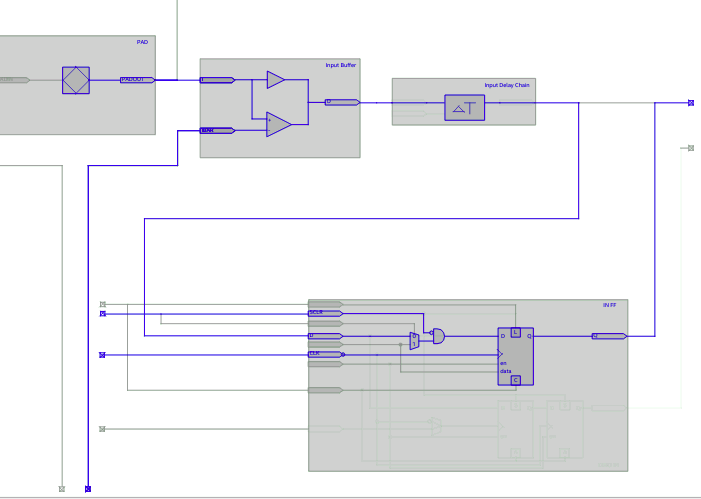
\includegraphics[width=0.8\linewidth]{images/quartus/fastinputregister-quartus}
    \caption{Input register}
    \label{fig:fastinputregister-quartus}
\end{figure} 

\begin{figure}[htb]
    \centering
    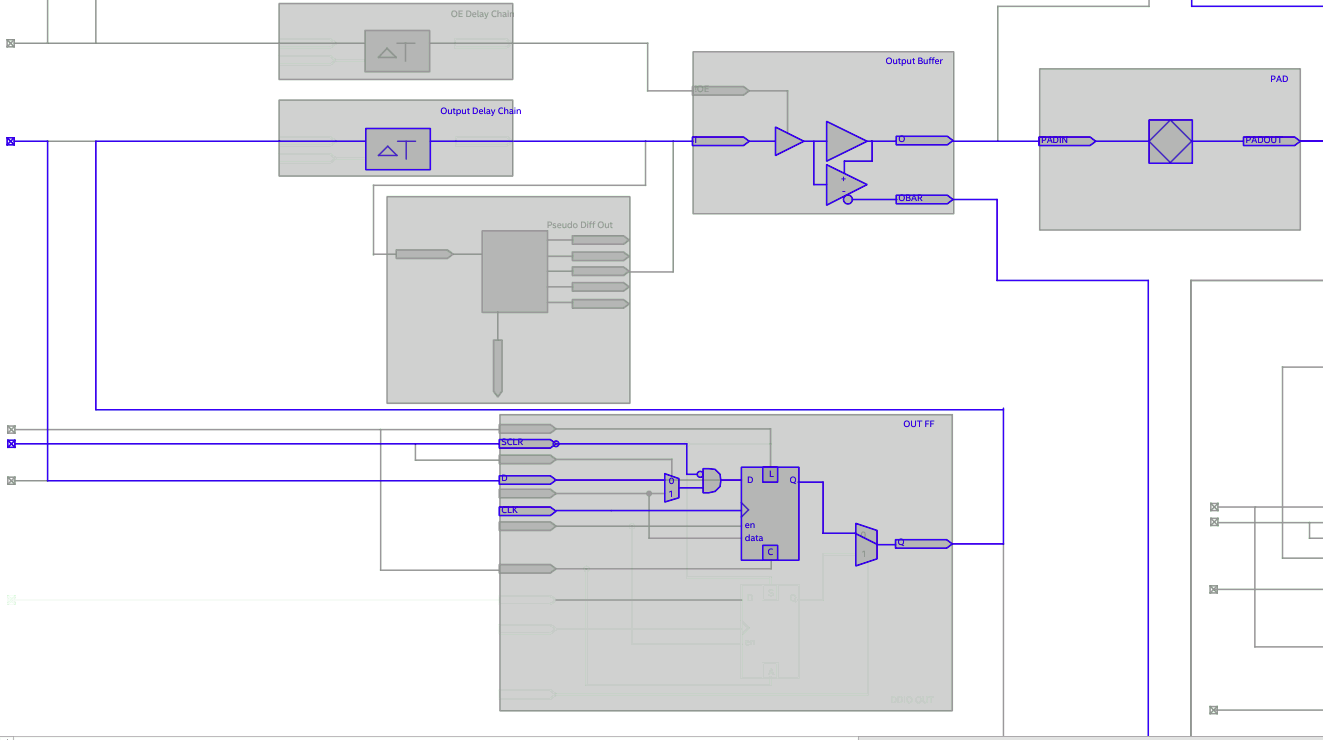
\includegraphics[width=0.8\linewidth]{images/quartus/fastoutputregister-quartus}
    \caption{Output register}
    \label{fig:fastoutputregister-quartus}
\end{figure} 


\begin{listing}[ht]
\begin{tclcode*}{}
set_instance_assignment -name FAST_INPUT_REGISTER ON -to path_to_register
set_instance_assignment -name FAST_OUPUT_REGISTER ON -to path_to_register
\end{tclcode*}
\caption{Intel fast registers QSF/TCL example}
\label{listing:fastregister}
\end{listing}

\begin{listing}[ht]
\begin{tclcode*}{}
set_property IOB TRUE [get_cells {path_to_register}]
\end{tclcode*}
\caption{Xilinx IOB registers XDC/TCL example}
\label{listing:iobregister}
\end{listing}

\subsection{Loosen I/O delay constraints}

One may not need to constraint the I/O if dedicated registers are used. The skew will be very low because the I/O pads have direct access to the clock tree. The clock tree is designed to deliver the clock with very low skew to several parts of the FPGA. The clock skew is the time difference between the clock signal arriving at source and destination end-points in a given clock path, i.e. $t_{skew} = t_{destination} - t_{source}$. If positive, source receives the clock earlier than the destination. If negative, source receives the clock later than the destination. 

\Cref{listing:outputdelay} shows an Intel and Xilinx loosen output timing SDC/XDC/TCL example. Having minimum and maximum values to 0 means that there is no external delay, and the fitter can generate a design with $T_{co}$ within any value in $0 \leq T_{co} \leq T_{clk}$. As larger is the difference between minimum and maximum values for the I/O delay, more difficult is to close timing~\cite{scovilleTimeQuestUserGuide2010}. Notice that \textit{tx\_lvds*} translates to any bit of \textit{tx\_lvds} and the respective differential pair. \Cref{fig:Tcodatasheet-quartus.png} shows the clock-to-output times for all the \textit{tx\_lvds*} ports. Keep in mind that maximum $T_{co}$ values are shown by default. The minimum values are available in the \textit{Minimum clock to Output Times} tab. 

\begin{listing}[ht]
\begin{tclcode*}{}
# Virtual clock representing the clock of the external receiver
create_clock -period 6.25 -name ttc_clk_ext
# Minimum and maximum delay set to 0
set_output_delay -clock ttc_clk_ext -max 0.0 [get_ports tx_lvds*]
set_output_delay -clock ttc_clk_ext -min 0.0 [get_ports tx_lvds*]
\end{tclcode*}
\caption{Intel and Xilinx loosen output timing SDC/XDC/TCL example}
\label{listing:outputdelay}
\end{listing}

\begin{figure}[htb]
    \centering
    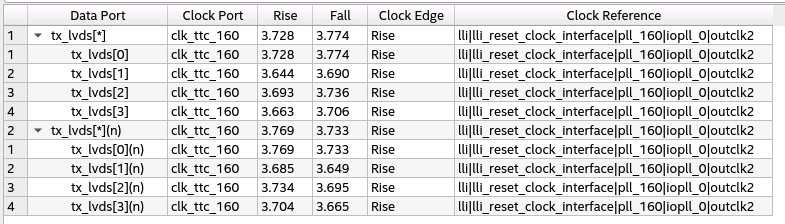
\includegraphics[width=1\linewidth]{images/quartus/Tcodatasheet-quartus.png}
    \caption{Clock to output times from Quartus Timing Analyzer datasheet report}
    \label{fig:Tcodatasheet-quartus.png}
\end{figure} 




\section{Clock groups}

For both Xilinx and Intel, by default, all clocks are related. So, clock groups are used to overwrite this default assumption.

This assumption is overwritten using the \textit{set\_clock\_groups} constraint. This defines groups of clocks that are inter-related but unrelated to other groups, regardless if these other groups are defined or not. 
 Then, here is the catch:
 
 \begin{itemize}
     \item \textbf{Option A:} Having 2 or more groups in the \textit{set\_clock\_groups} constraint means that the clocks within each group is related to each other and unrelated to the clocks defined in the other groups. 
     \item \textbf{Option B:} Having 1 group in the \textit{set\_clock\_groups} constraint means that the clocks within the group is related to each other and unrelated to ANY other clock, including clocks that have not been associated to a group by the user.
 \end{itemize}
 
 \Cref{listing:clockgroupsssdc,listing:clockgroupssxdc} show SDC and XDC clock groups examples. SDC and XDC are used for Intel and Xilinx designs, respectively. 
 
 \begin{listing}[ht]
\begin{tclcode*}{}
# Assign adc_clk, clocks generated from adc_clk and sys_clk, clocks generated from sys_clk to different clock groups
set_clock_groups -asynchronous \
-group [get_clocks {adc_clk \
the_adc_pll|Intel FPGA IOPLL_component_autogenerated|pll|clk[0] \
the_adc_pll|Intel FPGA IOPLL_component_autogenerated|pll|clk[1] \
the_adc_pll|Intel FPGA IOPLL_component_autogenerated|pll|clk[2] \
}] \
-group [get_clock {sys_clk \
the_system_pll|Intel FPGA IOPLL_component_autogenerated|pll|clk[0] \
the_system_pll|Intel FPGA IOPLL_component_autogenerated|pll|clk[1] \
}]
\end{tclcode*}
\caption{Intel clock groups SDC example}
\label{listing:clockgroupssdc}
\end{listing}

 \begin{listing}[ht]
\begin{tclcode*}{}
# Assign adc_clk, clocks generated from adc_clk and sys_clk, clocks generated from sys_clk to different clock groups
set_clock_groups -asynchronous \
-group [get_clocks -include_generated_clocks adc_clk] \
-group [get_clocks -include_generated_clocks sys_clk]
\end{tclcode*}
\caption{Xilinx clock groups XDC example}
\label{listing:clockgroupssxdc}
\end{listing}

\subsection{One or multiple \textit{set\_clock\_groups} statements?}

Here comes the bit danger part, if you create a new output in a PLL and forget to add to the respective clock group, you have different outcomes depending if you used a single statement clock group or multiple statements. 

 \begin{itemize}
     \item \textbf{Option B:} If you used one \textit{set\_clock\_groups} statement per group, all the clocks belonging to these groups will be unrelated to this new generated clock. This happens because you have set they would be unrelated to ANY other clock, including clocks that do not belong to a user-specified group. 
     \item \textbf{Option A:} If you used a single \textit{set\_clock\_groups} statement for all groups, all these clocks groups will be unrelated to each other, but related to a clock that is not specified to any of these groups. Having 2 or more groups do not impose the non-relationship to any other clock. 
 \end{itemize}

Going for option A is always safer, because if you forget to update your clock groups, this new generated clock inherits the default assumption of being related, so handled by static timing analysis. 

Limiting the scope to Xilinx, Vivado offers the option of using the option \textit{-include\_generated\_clocks} to~ the base clock,  then all the generated clocks would be included automatically to their base clock group. 
This way, one could still specify clock groups using multiple statements with reasonable robustness. So, in principle, for Xilinx designs one could still choose options A or B if using the option \textit{-include\_generated\_clocks}.

As you said, specifying two clocks as unrelated, means to have a set\_false\_path between any end-points from clock A to B and vice-versa. And this should be done if clocks are unrelated. 


\cleardoublepage
%-------------------------------------------------------------------------------
% References
%-------------------------------------------------------------------------------
\pagestyle{ATLASPhaseIIBib}
\phantomsection  % this is needed for the correct links in the pdf (e.g. pdfviewer)
\addcontentsline{toc}{chapter}{\bibname}
\printbibliography[heading=subbibliography]   % subbibintoc is needed for the reference to look as a section and not a chapter
\label{pg:lastpage}
\clearpage

%-------------------------------------------------------------------------------
% Appendix
%-------------------------------------------------------------------------------
\begin{appendices}
\backmatter
\include{text/Appendix}

\chapter{Terms, Definitions and Glossary}
\label{cha:terms}

\listofdefinition
\listofrequirement
\listofspecification
\listofrecommendation
\listofremark
\listoftables
\listoffigures
%-------------------------------------------------------------------------------
% Glossary (list of acronyms)
%-------------------------------------------------------------------------------
\section{Glossary}
\label{sec:glossary}
\renewcommand{\glossarysection}[2][]{}
% optionally print all glossary entries (the unused ones) - not recommended
%\glsaddallunused
\printglossary[type=main]

\clearpage
\end{appendices}

\end{document}
